\documentclass[1p]{elsarticle_modified}
%\bibliographystyle{elsarticle-num}

%\usepackage[colorlinks]{hyperref}
%\usepackage{abbrmath_seonhwa} %\Abb, \Ascr, \Acal ,\Abf, \Afrak
\usepackage{amsfonts}
\usepackage{amssymb}
\usepackage{amsmath}
\usepackage{amsthm}
\usepackage{scalefnt}
\usepackage{amsbsy}
\usepackage{kotex}
\usepackage{caption}
\usepackage{subfig}
\usepackage{color}
\usepackage{graphicx}
\usepackage{xcolor} %% white, black, red, green, blue, cyan, magenta, yellow
\usepackage{float}
\usepackage{setspace}
\usepackage{hyperref}

\usepackage{tikz}
\usetikzlibrary{arrows}

\usepackage{multirow}
\usepackage{array} % fixed length table
\usepackage{hhline}

%%%%%%%%%%%%%%%%%%%%%
\makeatletter
\renewcommand*\env@matrix[1][\arraystretch]{%
	\edef\arraystretch{#1}%
	\hskip -\arraycolsep
	\let\@ifnextchar\new@ifnextchar
	\array{*\c@MaxMatrixCols c}}
\makeatother %https://tex.stackexchange.com/questions/14071/how-can-i-increase-the-line-spacing-in-a-matrix
%%%%%%%%%%%%%%%

\usepackage[normalem]{ulem}

\newcommand{\msout}[1]{\ifmmode\text{\sout{\ensuremath{#1}}}\else\sout{#1}\fi}
%SOURCE: \msout is \stkout macro in https://tex.stackexchange.com/questions/20609/strikeout-in-math-mode

\newcommand{\cancel}[1]{
	\ifmmode
	{\color{red}\msout{#1}}
	\else
	{\color{red}\sout{#1}}
	\fi
}

\newcommand{\add}[1]{
	{\color{blue}\uwave{#1}}
}

\newcommand{\replace}[2]{
	\ifmmode
	{\color{red}\msout{#1}}{\color{blue}\uwave{#2}}
	\else
	{\color{red}\sout{#1}}{\color{blue}\uwave{#2}}
	\fi
}

\newcommand{\Sol}{\mathcal{S}} %segment
\newcommand{\D}{D} %diagram
\newcommand{\A}{\mathcal{A}} %arc


%%%%%%%%%%%%%%%%%%%%%%%%%%%%%5 test

\def\sl{\operatorname{\textup{SL}}(2,\Cbb)}
\def\psl{\operatorname{\textup{PSL}}(2,\Cbb)}
\def\quan{\mkern 1mu \triangleright \mkern 1mu}

\theoremstyle{definition}
\newtheorem{thm}{Theorem}[section]
\newtheorem{prop}[thm]{Proposition}
\newtheorem{lem}[thm]{Lemma}
\newtheorem{ques}[thm]{Question}
\newtheorem{cor}[thm]{Corollary}
\newtheorem{defn}[thm]{Definition}
\newtheorem{exam}[thm]{Example}
\newtheorem{rmk}[thm]{Remark}
\newtheorem{alg}[thm]{Algorithm}

\newcommand{\I}{\sqrt{-1}}
\begin{document}

%\begin{frontmatter}
%
%\title{Boundary parabolic representations of knots up to 8 crossings}
%
%%% Group authors per affiliation:
%\author{Yunhi Cho} 
%\address{Department of Mathematics, University of Seoul, Seoul, Korea}
%\ead{yhcho@uos.ac.kr}
%
%
%\author{Seonhwa Kim} %\fnref{s_kim}}
%\address{Center for Geometry and Physics, Institute for Basic Science, Pohang, 37673, Korea}
%\ead{ryeona17@ibs.re.kr}
%
%\author{Hyuk Kim}
%\address{Department of Mathematical Sciences, Seoul National University, Seoul 08826, Korea}
%\ead{hyukkim@snu.ac.kr}
%
%\author{Seokbeom Yoon}
%\address{Department of Mathematical Sciences, Seoul National University, Seoul, 08826,  Korea}
%\ead{sbyoon15@snu.ac.kr}
%
%\begin{abstract}
%We find all boundary parabolic representation of knots up to 8 crossings.
%
%\end{abstract}
%\begin{keyword}
%    \MSC[2010] 57M25 
%\end{keyword}
%
%\end{frontmatter}

%\linenumbers
%\tableofcontents
%
\newcommand\colored[1]{\textcolor{white}{\rule[-0.35ex]{0.8em}{1.4ex}}\kern-0.8em\color{red} #1}%
%\newcommand\colored[1]{\textcolor{white}{ #1}\kern-2.17ex	\textcolor{white}{ #1}\kern-1.81ex	\textcolor{white}{ #1}\kern-2.15ex\color{red}#1	}

{\Large $\underline{11a_{71}~(K11a_{71})}$}

\setlength{\tabcolsep}{10pt}
\renewcommand{\arraystretch}{1.6}
\vspace{1cm}\begin{tabular}{m{100pt}>{\centering\arraybackslash}m{274pt}}
\multirow{5}{120pt}{
	\centering
	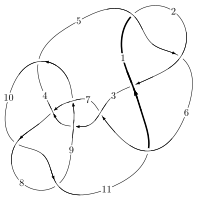
\includegraphics[width=112pt]{../../../GIT/diagram.site/Diagrams/png/320_11a_71.png}\\
\ \ \ A knot diagram\footnotemark}&
\allowdisplaybreaks
\textbf{Linearized knot diagam} \\
\cline{2-2}
 &
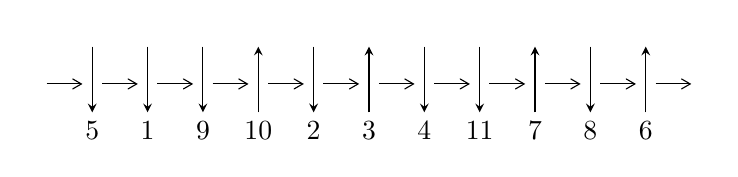
\begin{tikzpicture}[x=20pt, y=17pt]
	% nodes
	\node (C0) at (0, 0) {};
	\node (C1) at (1, 0) {};
	\node (C1U) at (1, +1) {};
	\node (C1D) at (1, -1) {5};

	\node (C2) at (2, 0) {};
	\node (C2U) at (2, +1) {};
	\node (C2D) at (2, -1) {1};

	\node (C3) at (3, 0) {};
	\node (C3U) at (3, +1) {};
	\node (C3D) at (3, -1) {9};

	\node (C4) at (4, 0) {};
	\node (C4U) at (4, +1) {};
	\node (C4D) at (4, -1) {10};

	\node (C5) at (5, 0) {};
	\node (C5U) at (5, +1) {};
	\node (C5D) at (5, -1) {2};

	\node (C6) at (6, 0) {};
	\node (C6U) at (6, +1) {};
	\node (C6D) at (6, -1) {3};

	\node (C7) at (7, 0) {};
	\node (C7U) at (7, +1) {};
	\node (C7D) at (7, -1) {4};

	\node (C8) at (8, 0) {};
	\node (C8U) at (8, +1) {};
	\node (C8D) at (8, -1) {11};

	\node (C9) at (9, 0) {};
	\node (C9U) at (9, +1) {};
	\node (C9D) at (9, -1) {7};

	\node (C10) at (10, 0) {};
	\node (C10U) at (10, +1) {};
	\node (C10D) at (10, -1) {8};

	\node (C11) at (11, 0) {};
	\node (C11U) at (11, +1) {};
	\node (C11D) at (11, -1) {6};
	\node (C12) at (12, 0) {};

	% arrows
	\draw[->,>={angle 60}]
	(C0) edge (C1) (C1) edge (C2) (C2) edge (C3) (C3) edge (C4) (C4) edge (C5) (C5) edge (C6) (C6) edge (C7) (C7) edge (C8) (C8) edge (C9) (C9) edge (C10) (C10) edge (C11) (C11) edge (C12) ;	\draw[->,>=stealth]
	(C1U) edge (C1D) (C2U) edge (C2D) (C3U) edge (C3D) (C4D) edge (C4U) (C5U) edge (C5D) (C6D) edge (C6U) (C7U) edge (C7D) (C8U) edge (C8D) (C9D) edge (C9U) (C10U) edge (C10D) (C11D) edge (C11U) ;
	\end{tikzpicture} \\
\hhline{~~} \\& 
\textbf{Solving Sequence} \\ \cline{2-2} 
 &
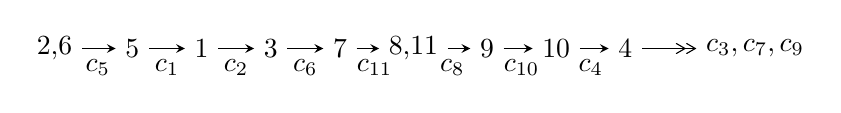
\begin{tikzpicture}[x=25pt, y=7pt]
	% node
	\node (A0) at (-1/8, 0) {2,6};
	\node (A1) at (1, 0) {5};
	\node (A2) at (2, 0) {1};
	\node (A3) at (3, 0) {3};
	\node (A4) at (4, 0) {7};
	\node (A5) at (81/16, 0) {8,11};
	\node (A6) at (49/8, 0) {9};
	\node (A7) at (57/8, 0) {10};
	\node (A8) at (65/8, 0) {4};
	\node (C1) at (1/2, -1) {$c_{5}$};
	\node (C2) at (3/2, -1) {$c_{1}$};
	\node (C3) at (5/2, -1) {$c_{2}$};
	\node (C4) at (7/2, -1) {$c_{6}$};
	\node (C5) at (9/2, -1) {$c_{11}$};
	\node (C6) at (45/8, -1) {$c_{8}$};
	\node (C7) at (53/8, -1) {$c_{10}$};
	\node (C8) at (61/8, -1) {$c_{4}$};
	\node (A9) at (10, 0) {$c_{3},c_{7},c_{9}$};

	% edge
	\draw[->,>=stealth]	
	(A0) edge (A1) (A1) edge (A2) (A2) edge (A3) (A3) edge (A4) (A4) edge (A5) (A5) edge (A6) (A6) edge (A7) (A7) edge (A8) ;
	\draw[->>,>={angle 60}]	
	(A8) edge (A9);
\end{tikzpicture} \\ 

\end{tabular} \\

\footnotetext{
The image of knot diagram is generated by the software ``\textbf{Draw programme}" developed by Andrew Bartholomew(\url{http://www.layer8.co.uk/maths/draw/index.htm\#Running-draw}), where we modified some parts for our purpose(\url{https://github.com/CATsTAILs/LinksPainter}).
}\phantom \\ \newline 
\centering \textbf{Ideals for irreducible components\footnotemark of $X_{\text{par}}$} 
 
\begin{align*}
I^u_{1}&=\langle 
7.83384\times10^{25} u^{79}-2.56733\times10^{25} u^{78}+\cdots+1.29163\times10^{26} b-2.49920\times10^{25},\\
\phantom{I^u_{1}}&\phantom{= \langle  }2.29485\times10^{26} u^{79}+3.32810\times10^{26} u^{78}+\cdots+6.45815\times10^{25} a+5.38395\times10^{26},\;u^{80}+2 u^{79}+\cdots+5 u+1\rangle \\
I^u_{2}&=\langle 
b-1,\;a+1,\;u+1\rangle \\
\\
\end{align*}
\raggedright * 2 irreducible components of $\dim_{\mathbb{C}}=0$, with total 81 representations.\\
\footnotetext{All coefficients of polynomials are rational numbers. But the coefficients are sometimes approximated in decimal forms when there is not enough margin.}
\newpage
\renewcommand{\arraystretch}{1}
\centering \section*{I. $I^u_{1}= \langle 7.83\times10^{25} u^{79}-2.57\times10^{25} u^{78}+\cdots+1.29\times10^{26} b-2.50\times10^{25},\;2.29\times10^{26} u^{79}+3.33\times10^{26} u^{78}+\cdots+6.46\times10^{25} a+5.38\times10^{26},\;u^{80}+2 u^{79}+\cdots+5 u+1 \rangle$}
\flushleft \textbf{(i) Arc colorings}\\
\begin{tabular}{m{7pt} m{180pt} m{7pt} m{180pt} }
\flushright $a_{2}=$&$\begin{pmatrix}0\\u\end{pmatrix}$ \\
\flushright $a_{6}=$&$\begin{pmatrix}1\\0\end{pmatrix}$ \\
\flushright $a_{5}=$&$\begin{pmatrix}1\\- u^2\end{pmatrix}$ \\
\flushright $a_{1}=$&$\begin{pmatrix}u\\- u^3+u\end{pmatrix}$ \\
\flushright $a_{3}=$&$\begin{pmatrix}- u^3\\u^5- u^3+u\end{pmatrix}$ \\
\flushright $a_{7}=$&$\begin{pmatrix}u^8- u^6+u^4+1\\- u^{10}+2 u^8-3 u^6+2 u^4- u^2\end{pmatrix}$ \\
\flushright $a_{8}=$&$\begin{pmatrix}-3.55341 u^{79}-5.15334 u^{78}+\cdots-20.1149 u-8.33667\\-0.606508 u^{79}+0.198767 u^{78}+\cdots+0.990713 u+0.193492\end{pmatrix}$ \\
\flushright $a_{11}=$&$\begin{pmatrix}u^3\\- u^3+u\end{pmatrix}$ \\
\flushright $a_{9}=$&$\begin{pmatrix}-3.78703 u^{79}-5.38668 u^{78}+\cdots-20.9985 u-8.55334\\-0.572619 u^{79}+0.249326 u^{78}+\cdots+1.94321 u+0.227381\end{pmatrix}$ \\
\flushright $a_{10}=$&$\begin{pmatrix}-4.01996 u^{79}-5.62000 u^{78}+\cdots-20.4242 u-8.87000\\-0.540079 u^{79}+0.255493 u^{78}+\cdots+1.98965 u+0.259921\end{pmatrix}$ \\
\flushright $a_{4}=$&$\begin{pmatrix}8.92076 u^{79}+10.5265 u^{78}+\cdots+40.2493 u+13.8432\\-1.55419 u^{79}-2.35995 u^{78}+\cdots-9.35652 u-2.35995\end{pmatrix}$\\ \flushright $a_{4}=$&$\begin{pmatrix}8.92076 u^{79}+10.5265 u^{78}+\cdots+40.2493 u+13.8432\\-1.55419 u^{79}-2.35995 u^{78}+\cdots-9.35652 u-2.35995\end{pmatrix}$\\&\end{tabular}
\flushleft \textbf{(ii) Obstruction class $= -1$}\\~\\
\flushleft \textbf{(iii) Cusp Shapes $= -\frac{120968554523544040789727864}{21527170222575090764609709} u^{79}-\frac{5739563596393551567527518}{1025103343932147179267129} u^{78}+\cdots-\frac{240609495551769451833935926}{7175723407525030254869903} u-\frac{236354186912654203058622196}{21527170222575090764609709}$}\\~\\
\newpage\renewcommand{\arraystretch}{1}
\flushleft \textbf{(iv) u-Polynomials at the component}\newline \\
\begin{tabular}{m{50pt}|m{274pt}}
Crossings & \hspace{64pt}u-Polynomials at each crossing \\
\hline $$\begin{aligned}c_{1},c_{5}\end{aligned}$$&$\begin{aligned}
&u^{80}+2 u^{79}+\cdots+5 u+1
\end{aligned}$\\
\hline $$\begin{aligned}c_{2}\end{aligned}$$&$\begin{aligned}
&u^{80}+38 u^{79}+\cdots+5 u+1
\end{aligned}$\\
\hline $$\begin{aligned}c_{3}\end{aligned}$$&$\begin{aligned}
&u^{80}+35 u^{78}+\cdots+27 u-1
\end{aligned}$\\
\hline $$\begin{aligned}c_{4}\end{aligned}$$&$\begin{aligned}
&u^{80}+2 u^{79}+\cdots+89 u+19
\end{aligned}$\\
\hline $$\begin{aligned}c_{6}\end{aligned}$$&$\begin{aligned}
&u^{80}-15 u^{78}+\cdots+56453 u+8017
\end{aligned}$\\
\hline $$\begin{aligned}c_{7}\end{aligned}$$&$\begin{aligned}
&u^{80}+4 u^{79}+\cdots- u-1
\end{aligned}$\\
\hline $$\begin{aligned}c_{8},c_{10}\end{aligned}$$&$\begin{aligned}
&u^{80}-2 u^{79}+\cdots+5 u-1
\end{aligned}$\\
\hline $$\begin{aligned}c_{9}\end{aligned}$$&$\begin{aligned}
&u^{80}+13 u^{79}+\cdots+6 u+2
\end{aligned}$\\
\hline $$\begin{aligned}c_{11}\end{aligned}$$&$\begin{aligned}
&u^{80}+3 u^{79}+\cdots-1824 u-288
\end{aligned}$\\
\hline
\end{tabular}\\~\\
\newpage\renewcommand{\arraystretch}{1}
\flushleft \textbf{(v) Riley Polynomials at the component}\newline \\
\begin{tabular}{m{50pt}|m{274pt}}
Crossings & \hspace{64pt}Riley Polynomials at each crossing \\
\hline $$\begin{aligned}c_{1},c_{5}\end{aligned}$$&$\begin{aligned}
&y^{80}-38 y^{79}+\cdots-5 y+1
\end{aligned}$\\
\hline $$\begin{aligned}c_{2}\end{aligned}$$&$\begin{aligned}
&y^{80}+10 y^{79}+\cdots-73 y+1
\end{aligned}$\\
\hline $$\begin{aligned}c_{3}\end{aligned}$$&$\begin{aligned}
&y^{80}+70 y^{79}+\cdots-129 y+1
\end{aligned}$\\
\hline $$\begin{aligned}c_{4}\end{aligned}$$&$\begin{aligned}
&y^{80}+78 y^{79}+\cdots+10547 y+361
\end{aligned}$\\
\hline $$\begin{aligned}c_{6}\end{aligned}$$&$\begin{aligned}
&y^{80}-30 y^{79}+\cdots-2160187985 y+64272289
\end{aligned}$\\
\hline $$\begin{aligned}c_{7}\end{aligned}$$&$\begin{aligned}
&y^{80}-14 y^{79}+\cdots-5 y+1
\end{aligned}$\\
\hline $$\begin{aligned}c_{8},c_{10}\end{aligned}$$&$\begin{aligned}
&y^{80}-50 y^{79}+\cdots+55 y+1
\end{aligned}$\\
\hline $$\begin{aligned}c_{9}\end{aligned}$$&$\begin{aligned}
&y^{80}-9 y^{79}+\cdots-64 y+4
\end{aligned}$\\
\hline $$\begin{aligned}c_{11}\end{aligned}$$&$\begin{aligned}
&y^{80}+15 y^{79}+\cdots+2084544 y+82944
\end{aligned}$\\
\hline
\end{tabular}\\~\\
\newpage\flushleft \textbf{(vi) Complex Volumes and Cusp Shapes}
$$\begin{array}{c|c|c}  
\text{Solutions to }I^u_{1}& \I (\text{vol} + \sqrt{-1}CS) & \text{Cusp shape}\\
 \hline 
\begin{aligned}
u &= -0.993582 + 0.219652 I \\
a &= -0.681629 + 0.056586 I \\
b &= -0.017242 - 0.156551 I\end{aligned}
 & -1.76831 + 0.41384 I & \phantom{-0.000000 } 0 \\ \hline\begin{aligned}
u &= -0.993582 - 0.219652 I \\
a &= -0.681629 - 0.056586 I \\
b &= -0.017242 + 0.156551 I\end{aligned}
 & -1.76831 - 0.41384 I & \phantom{-0.000000 } 0 \\ \hline\begin{aligned}
u &= -0.633725 + 0.710008 I \\
a &= \phantom{-}1.304580 + 0.456964 I \\
b &= -1.169060 - 0.469516 I\end{aligned}
 & \phantom{-}1.10017 + 9.52896 I & \phantom{-0.000000 } 0. - 7.63149 I \\ \hline\begin{aligned}
u &= -0.633725 - 0.710008 I \\
a &= \phantom{-}1.304580 - 0.456964 I \\
b &= -1.169060 + 0.469516 I\end{aligned}
 & \phantom{-}1.10017 - 9.52896 I & \phantom{-0.000000 -}0. + 7.63149 I \\ \hline\begin{aligned}
u &= \phantom{-}0.666948 + 0.650580 I \\
a &= -1.033680 + 0.452004 I \\
b &= \phantom{-}1.264010 - 0.241396 I\end{aligned}
 & \phantom{-}2.84471 - 1.91218 I & \phantom{-}3.52882 + 5.17190 I \\ \hline\begin{aligned}
u &= \phantom{-}0.666948 - 0.650580 I \\
a &= -1.033680 - 0.452004 I \\
b &= \phantom{-}1.264010 + 0.241396 I\end{aligned}
 & \phantom{-}2.84471 + 1.91218 I & \phantom{-}3.52882 - 5.17190 I \\ \hline\begin{aligned}
u &= -1.031480 + 0.286770 I \\
a &= \phantom{-}0.53377 - 6.02234 I \\
b &= \phantom{-}3.13018 + 2.41426 I\end{aligned}
 & -3.78449 + 0.73170 I & \phantom{-0.000000 } 0 \\ \hline\begin{aligned}
u &= -1.031480 - 0.286770 I \\
a &= \phantom{-}0.53377 + 6.02234 I \\
b &= \phantom{-}3.13018 - 2.41426 I\end{aligned}
 & -3.78449 - 0.73170 I & \phantom{-0.000000 } 0 \\ \hline\begin{aligned}
u &= -1.017560 + 0.366491 I \\
a &= \phantom{-}0.142352 + 1.380120 I \\
b &= -0.580624 - 0.069040 I\end{aligned}
 & -2.69872 + 1.44530 I & \phantom{-0.000000 } 0 \\ \hline\begin{aligned}
u &= -1.017560 - 0.366491 I \\
a &= \phantom{-}0.142352 - 1.380120 I \\
b &= -0.580624 + 0.069040 I\end{aligned}
 & -2.69872 - 1.44530 I & \phantom{-0.000000 } 0\\
 \hline 
 \end{array}$$\newpage$$\begin{array}{c|c|c}  
\text{Solutions to }I^u_{1}& \I (\text{vol} + \sqrt{-1}CS) & \text{Cusp shape}\\
 \hline 
\begin{aligned}
u &= \phantom{-}0.529228 + 0.750028 I \\
a &= -0.766967 + 0.360768 I \\
b &= \phantom{-}0.522843 + 0.472910 I\end{aligned}
 & \phantom{-}3.02838 + 1.37936 I & \phantom{-}3.64616 - 3.11353 I \\ \hline\begin{aligned}
u &= \phantom{-}0.529228 - 0.750028 I \\
a &= -0.766967 - 0.360768 I \\
b &= \phantom{-}0.522843 - 0.472910 I\end{aligned}
 & \phantom{-}3.02838 - 1.37936 I & \phantom{-}3.64616 + 3.11353 I \\ \hline\begin{aligned}
u &= \phantom{-}0.924365 + 0.563218 I \\
a &= -0.78920 + 1.35114 I \\
b &= \phantom{-}1.063890 - 0.643299 I\end{aligned}
 & \phantom{-}2.08735 - 2.83654 I & \phantom{-0.000000 } 0 \\ \hline\begin{aligned}
u &= \phantom{-}0.924365 - 0.563218 I \\
a &= -0.78920 - 1.35114 I \\
b &= \phantom{-}1.063890 + 0.643299 I\end{aligned}
 & \phantom{-}2.08735 + 2.83654 I & \phantom{-0.000000 } 0 \\ \hline\begin{aligned}
u &= \phantom{-}1.085720 + 0.197443 I \\
a &= -0.544690 - 0.850906 I \\
b &= \phantom{-}0.308390 + 1.048710 I\end{aligned}
 & -1.19443 + 3.73477 I & \phantom{-0.000000 } 0 \\ \hline\begin{aligned}
u &= \phantom{-}1.085720 - 0.197443 I \\
a &= -0.544690 + 0.850906 I \\
b &= \phantom{-}0.308390 - 1.048710 I\end{aligned}
 & -1.19443 - 3.73477 I & \phantom{-0.000000 } 0 \\ \hline\begin{aligned}
u &= \phantom{-}1.078910 + 0.266597 I \\
a &= -0.12207 - 2.82977 I \\
b &= -1.45556 + 1.85197 I\end{aligned}
 & -5.69690 + 1.47728 I & \phantom{-0.000000 } 0 \\ \hline\begin{aligned}
u &= \phantom{-}1.078910 - 0.266597 I \\
a &= -0.12207 + 2.82977 I \\
b &= -1.45556 - 1.85197 I\end{aligned}
 & -5.69690 - 1.47728 I & \phantom{-0.000000 } 0 \\ \hline\begin{aligned}
u &= -0.562648 + 0.677266 I \\
a &= \phantom{-}0.225635 + 0.785522 I \\
b &= -0.233404 + 0.503707 I\end{aligned}
 & \phantom{-}4.34092 + 3.75201 I & \phantom{-}2.40820 - 5.29181 I \\ \hline\begin{aligned}
u &= -0.562648 - 0.677266 I \\
a &= \phantom{-}0.225635 - 0.785522 I \\
b &= -0.233404 - 0.503707 I\end{aligned}
 & \phantom{-}4.34092 - 3.75201 I & \phantom{-}2.40820 + 5.29181 I\\
 \hline 
 \end{array}$$\newpage$$\begin{array}{c|c|c}  
\text{Solutions to }I^u_{1}& \I (\text{vol} + \sqrt{-1}CS) & \text{Cusp shape}\\
 \hline 
\begin{aligned}
u &= \phantom{-}1.075990 + 0.321255 I \\
a &= -0.12764 - 2.13134 I \\
b &= -1.77154 + 1.40590 I\end{aligned}
 & -6.18593 - 2.21505 I & \phantom{-0.000000 } 0 \\ \hline\begin{aligned}
u &= \phantom{-}1.075990 - 0.321255 I \\
a &= -0.12764 + 2.13134 I \\
b &= -1.77154 - 1.40590 I\end{aligned}
 & -6.18593 + 2.21505 I & \phantom{-0.000000 } 0 \\ \hline\begin{aligned}
u &= -0.358068 + 0.799824 I \\
a &= \phantom{-}1.125740 - 0.036921 I \\
b &= -0.45145 + 2.59579 I\end{aligned}
 & -0.37727 - 12.19400 I & -2.40584 + 6.91147 I \\ \hline\begin{aligned}
u &= -0.358068 - 0.799824 I \\
a &= \phantom{-}1.125740 + 0.036921 I \\
b &= -0.45145 - 2.59579 I\end{aligned}
 & -0.37727 + 12.19400 I & -2.40584 - 6.91147 I \\ \hline\begin{aligned}
u &= \phantom{-}0.322943 + 0.804382 I \\
a &= -0.956715 - 0.093636 I \\
b &= \phantom{-}0.61338 + 2.12460 I\end{aligned}
 & \phantom{-}0.97731 + 4.20187 I & -0.27939 - 7.34151 I \\ \hline\begin{aligned}
u &= \phantom{-}0.322943 - 0.804382 I \\
a &= -0.956715 + 0.093636 I \\
b &= \phantom{-}0.61338 - 2.12460 I\end{aligned}
 & \phantom{-}0.97731 - 4.20187 I & -0.27939 + 7.34151 I \\ \hline\begin{aligned}
u &= -0.950417 + 0.625173 I \\
a &= \phantom{-}1.29330 + 0.99233 I \\
b &= -1.084190 - 0.511800 I\end{aligned}
 & \phantom{-}0.16239 - 4.42235 I & \phantom{-0.000000 } 0 \\ \hline\begin{aligned}
u &= -0.950417 - 0.625173 I \\
a &= \phantom{-}1.29330 - 0.99233 I \\
b &= -1.084190 + 0.511800 I\end{aligned}
 & \phantom{-}0.16239 + 4.42235 I & \phantom{-0.000000 } 0 \\ \hline\begin{aligned}
u &= \phantom{-}1.067680 + 0.392778 I \\
a &= \phantom{-}0.852018 + 0.414010 I \\
b &= -0.780612 - 0.671395 I\end{aligned}
 & -2.94524 - 4.81984 I & \phantom{-0.000000 } 0 \\ \hline\begin{aligned}
u &= \phantom{-}1.067680 - 0.392778 I \\
a &= \phantom{-}0.852018 - 0.414010 I \\
b &= -0.780612 + 0.671395 I\end{aligned}
 & -2.94524 + 4.81984 I & \phantom{-0.000000 } 0\\
 \hline 
 \end{array}$$\newpage$$\begin{array}{c|c|c}  
\text{Solutions to }I^u_{1}& \I (\text{vol} + \sqrt{-1}CS) & \text{Cusp shape}\\
 \hline 
\begin{aligned}
u &= \phantom{-}0.435068 + 0.737884 I \\
a &= -0.527799 - 0.057176 I \\
b &= \phantom{-}0.365706 + 0.271011 I\end{aligned}
 & \phantom{-}2.69064 + 1.31991 I & \phantom{-}2.13735 + 0.80724 I \\ \hline\begin{aligned}
u &= \phantom{-}0.435068 - 0.737884 I \\
a &= -0.527799 + 0.057176 I \\
b &= \phantom{-}0.365706 - 0.271011 I\end{aligned}
 & \phantom{-}2.69064 - 1.31991 I & \phantom{-}2.13735 - 0.80724 I \\ \hline\begin{aligned}
u &= -0.381093 + 0.751489 I \\
a &= \phantom{-}0.343576 - 0.594171 I \\
b &= \phantom{-}0.560845 - 0.405823 I\end{aligned}
 & \phantom{-}3.42648 - 6.07271 I & \phantom{-}0.67730 + 5.78894 I \\ \hline\begin{aligned}
u &= -0.381093 - 0.751489 I \\
a &= \phantom{-}0.343576 + 0.594171 I \\
b &= \phantom{-}0.560845 + 0.405823 I\end{aligned}
 & \phantom{-}3.42648 + 6.07271 I & \phantom{-}0.67730 - 5.78894 I \\ \hline\begin{aligned}
u &= -1.001240 + 0.581180 I \\
a &= -0.619113 + 0.338239 I \\
b &= -0.469007 - 0.810748 I\end{aligned}
 & \phantom{-}3.04528 + 1.12254 I & \phantom{-0.000000 } 0 \\ \hline\begin{aligned}
u &= -1.001240 - 0.581180 I \\
a &= -0.619113 - 0.338239 I \\
b &= -0.469007 + 0.810748 I\end{aligned}
 & \phantom{-}3.04528 - 1.12254 I & \phantom{-0.000000 } 0 \\ \hline\begin{aligned}
u &= -1.045000 + 0.507333 I \\
a &= -0.507155 + 0.270967 I \\
b &= -0.264182 + 0.152064 I\end{aligned}
 & -2.30319 + 1.88747 I & \phantom{-0.000000 } 0 \\ \hline\begin{aligned}
u &= -1.045000 - 0.507333 I \\
a &= -0.507155 - 0.270967 I \\
b &= -0.264182 - 0.152064 I\end{aligned}
 & -2.30319 - 1.88747 I & \phantom{-0.000000 } 0 \\ \hline\begin{aligned}
u &= \phantom{-}1.155910 + 0.191256 I \\
a &= \phantom{-}0.84276 + 2.60711 I \\
b &= \phantom{-}0.92267 - 1.69592 I\end{aligned}
 & -5.29538 + 9.47417 I & \phantom{-0.000000 } 0 \\ \hline\begin{aligned}
u &= \phantom{-}1.155910 - 0.191256 I \\
a &= \phantom{-}0.84276 - 2.60711 I \\
b &= \phantom{-}0.92267 + 1.69592 I\end{aligned}
 & -5.29538 - 9.47417 I & \phantom{-0.000000 } 0\\
 \hline 
 \end{array}$$\newpage$$\begin{array}{c|c|c}  
\text{Solutions to }I^u_{1}& \I (\text{vol} + \sqrt{-1}CS) & \text{Cusp shape}\\
 \hline 
\begin{aligned}
u &= -1.17701\phantom{ +0.000000I} \\
a &= -0.658231\phantom{ +0.000000I} \\
b &= -0.350023\phantom{ +0.000000I}\end{aligned}
 & -2.75709\phantom{ +0.000000I} & \phantom{-0.000000 } 0 \\ \hline\begin{aligned}
u &= \phantom{-}1.059010 + 0.544082 I \\
a &= \phantom{-}2.90298 - 0.23263 I \\
b &= -1.80671 - 1.04197 I\end{aligned}
 & -1.35793 - 4.93977 I & \phantom{-0.000000 } 0 \\ \hline\begin{aligned}
u &= \phantom{-}1.059010 - 0.544082 I \\
a &= \phantom{-}2.90298 + 0.23263 I \\
b &= -1.80671 + 1.04197 I\end{aligned}
 & -1.35793 + 4.93977 I & \phantom{-0.000000 } 0 \\ \hline\begin{aligned}
u &= \phantom{-}1.027730 + 0.623923 I \\
a &= \phantom{-}0.067095 + 0.674046 I \\
b &= \phantom{-}0.550499 - 0.967599 I\end{aligned}
 & \phantom{-}1.55978 - 6.58436 I & \phantom{-0.000000 } 0 \\ \hline\begin{aligned}
u &= \phantom{-}1.027730 - 0.623923 I \\
a &= \phantom{-}0.067095 - 0.674046 I \\
b &= \phantom{-}0.550499 + 0.967599 I\end{aligned}
 & \phantom{-}1.55978 + 6.58436 I & \phantom{-0.000000 } 0 \\ \hline\begin{aligned}
u &= -1.191150 + 0.227672 I \\
a &= -1.19083 + 2.01827 I \\
b &= -0.48127 - 1.42841 I\end{aligned}
 & -3.84602 - 1.16588 I & \phantom{-0.000000 } 0 \\ \hline\begin{aligned}
u &= -1.191150 - 0.227672 I \\
a &= -1.19083 - 2.01827 I \\
b &= -0.48127 + 1.42841 I\end{aligned}
 & -3.84602 + 1.16588 I & \phantom{-0.000000 } 0 \\ \hline\begin{aligned}
u &= -1.092080 + 0.530795 I \\
a &= \phantom{-}1.39607 - 1.94234 I \\
b &= \phantom{-}0.28338 + 2.77059 I\end{aligned}
 & -4.75974 + 4.95618 I & \phantom{-0.000000 } 0 \\ \hline\begin{aligned}
u &= -1.092080 - 0.530795 I \\
a &= \phantom{-}1.39607 + 1.94234 I \\
b &= \phantom{-}0.28338 - 2.77059 I\end{aligned}
 & -4.75974 - 4.95618 I & \phantom{-0.000000 } 0 \\ \hline\begin{aligned}
u &= \phantom{-}1.086100 + 0.555013 I \\
a &= -4.94326 - 3.14688 I \\
b &= \phantom{-}1.11810 + 5.15447 I\end{aligned}
 & -1.91081 - 6.16425 I & \phantom{-0.000000 } 0\\
 \hline 
 \end{array}$$\newpage$$\begin{array}{c|c|c}  
\text{Solutions to }I^u_{1}& \I (\text{vol} + \sqrt{-1}CS) & \text{Cusp shape}\\
 \hline 
\begin{aligned}
u &= \phantom{-}1.086100 - 0.555013 I \\
a &= -4.94326 + 3.14688 I \\
b &= \phantom{-}1.11810 - 5.15447 I\end{aligned}
 & -1.91081 + 6.16425 I & \phantom{-0.000000 } 0 \\ \hline\begin{aligned}
u &= -0.349116 + 0.697052 I \\
a &= -0.850598 - 0.586037 I \\
b &= \phantom{-}0.15313 - 1.96985 I\end{aligned}
 & -1.57621 - 3.96915 I & -5.87435 + 6.27693 I \\ \hline\begin{aligned}
u &= -0.349116 - 0.697052 I \\
a &= -0.850598 + 0.586037 I \\
b &= \phantom{-}0.15313 + 1.96985 I\end{aligned}
 & -1.57621 + 3.96915 I & -5.87435 - 6.27693 I \\ \hline\begin{aligned}
u &= \phantom{-}0.393973 + 0.671200 I \\
a &= \phantom{-}1.57723 + 0.77061 I \\
b &= \phantom{-}0.38961 - 3.89569 I\end{aligned}
 & \phantom{-}0.103983 + 1.397740 I & \phantom{-}2.4292 + 14.3351 I \\ \hline\begin{aligned}
u &= \phantom{-}0.393973 - 0.671200 I \\
a &= \phantom{-}1.57723 - 0.77061 I \\
b &= \phantom{-}0.38961 + 3.89569 I\end{aligned}
 & \phantom{-}0.103983 - 1.397740 I & \phantom{-}2.4292 - 14.3351 I \\ \hline\begin{aligned}
u &= \phantom{-}0.457682 + 0.625241 I \\
a &= \phantom{-}0.565879 - 1.280020 I \\
b &= -1.18834 + 1.90703 I\end{aligned}
 & \phantom{-}0.412068 + 0.321069 I & -4.01206 - 8.91676 I \\ \hline\begin{aligned}
u &= \phantom{-}0.457682 - 0.625241 I \\
a &= \phantom{-}0.565879 + 1.280020 I \\
b &= -1.18834 - 1.90703 I\end{aligned}
 & \phantom{-}0.412068 - 0.321069 I & -4.01206 + 8.91676 I \\ \hline\begin{aligned}
u &= -0.527849 + 0.562689 I \\
a &= -1.116260 + 0.212682 I \\
b &= \phantom{-}0.123198 + 0.451359 I\end{aligned}
 & -0.74428 + 2.39884 I & -3.80212 - 6.62818 I \\ \hline\begin{aligned}
u &= -0.527849 - 0.562689 I \\
a &= -1.116260 - 0.212682 I \\
b &= \phantom{-}0.123198 - 0.451359 I\end{aligned}
 & -0.74428 - 2.39884 I & -3.80212 + 6.62818 I \\ \hline\begin{aligned}
u &= \phantom{-}1.087300 + 0.584528 I \\
a &= -0.135380 + 0.626345 I \\
b &= \phantom{-}0.248701 - 0.450700 I\end{aligned}
 & \phantom{-}0.75605 - 6.35925 I & \phantom{-0.000000 } 0\\
 \hline 
 \end{array}$$\newpage$$\begin{array}{c|c|c}  
\text{Solutions to }I^u_{1}& \I (\text{vol} + \sqrt{-1}CS) & \text{Cusp shape}\\
 \hline 
\begin{aligned}
u &= \phantom{-}1.087300 - 0.584528 I \\
a &= -0.135380 - 0.626345 I \\
b &= \phantom{-}0.248701 + 0.450700 I\end{aligned}
 & \phantom{-}0.75605 + 6.35925 I & \phantom{-0.000000 } 0 \\ \hline\begin{aligned}
u &= \phantom{-}1.165950 + 0.406590 I \\
a &= \phantom{-}1.22632 + 2.77362 I \\
b &= \phantom{-}1.06424 - 2.33151 I\end{aligned}
 & -7.89762 - 8.83460 I & \phantom{-0.000000 } 0 \\ \hline\begin{aligned}
u &= \phantom{-}1.165950 - 0.406590 I \\
a &= \phantom{-}1.22632 - 2.77362 I \\
b &= \phantom{-}1.06424 + 2.33151 I\end{aligned}
 & -7.89762 + 8.83460 I & \phantom{-0.000000 } 0 \\ \hline\begin{aligned}
u &= -1.103750 + 0.554364 I \\
a &= \phantom{-}2.12163 - 1.90495 I \\
b &= \phantom{-}0.24110 + 2.88334 I\end{aligned}
 & -3.76245 + 8.78286 I & \phantom{-0.000000 } 0 \\ \hline\begin{aligned}
u &= -1.103750 - 0.554364 I \\
a &= \phantom{-}2.12163 + 1.90495 I \\
b &= \phantom{-}0.24110 - 2.88334 I\end{aligned}
 & -3.76245 - 8.78286 I & \phantom{-0.000000 } 0 \\ \hline\begin{aligned}
u &= -1.107910 + 0.578539 I \\
a &= \phantom{-}0.099912 - 0.828642 I \\
b &= \phantom{-}0.979490 + 0.450273 I\end{aligned}
 & \phantom{-}1.28682 + 11.11430 I & \phantom{-0.000000 } 0 \\ \hline\begin{aligned}
u &= -1.107910 - 0.578539 I \\
a &= \phantom{-}0.099912 + 0.828642 I \\
b &= \phantom{-}0.979490 - 0.450273 I\end{aligned}
 & \phantom{-}1.28682 - 11.11430 I & \phantom{-0.000000 } 0 \\ \hline\begin{aligned}
u &= -0.042883 + 0.748508 I \\
a &= \phantom{-}0.389740 + 0.269401 I \\
b &= \phantom{-}0.15170 + 2.06876 I\end{aligned}
 & -4.35199 + 4.81540 I & -6.00555 - 5.45939 I \\ \hline\begin{aligned}
u &= -0.042883 - 0.748508 I \\
a &= \phantom{-}0.389740 - 0.269401 I \\
b &= \phantom{-}0.15170 - 2.06876 I\end{aligned}
 & -4.35199 - 4.81540 I & -6.00555 + 5.45939 I \\ \hline\begin{aligned}
u &= -1.169170 + 0.443646 I \\
a &= -1.65396 + 2.53789 I \\
b &= -0.39135 - 2.65142 I\end{aligned}
 & -7.65032 - 0.52064 I & \phantom{-0.000000 } 0\\
 \hline 
 \end{array}$$\newpage$$\begin{array}{c|c|c}  
\text{Solutions to }I^u_{1}& \I (\text{vol} + \sqrt{-1}CS) & \text{Cusp shape}\\
 \hline 
\begin{aligned}
u &= -1.169170 - 0.443646 I \\
a &= -1.65396 - 2.53789 I \\
b &= -0.39135 + 2.65142 I\end{aligned}
 & -7.65032 + 0.52064 I & \phantom{-0.000000 } 0 \\ \hline\begin{aligned}
u &= -1.130220 + 0.587955 I \\
a &= -2.32464 + 2.60165 I \\
b &= -0.18193 - 3.46366 I\end{aligned}
 & -2.6682 + 17.3873 I & \phantom{-0.000000 } 0 \\ \hline\begin{aligned}
u &= -1.130220 - 0.587955 I \\
a &= -2.32464 - 2.60165 I \\
b &= -0.18193 + 3.46366 I\end{aligned}
 & -2.6682 - 17.3873 I & \phantom{-0.000000 } 0 \\ \hline\begin{aligned}
u &= \phantom{-}1.142030 + 0.580131 I \\
a &= \phantom{-}1.67421 + 2.51891 I \\
b &= \phantom{-}0.39837 - 2.90345 I\end{aligned}
 & -1.44455 - 9.36809 I & \phantom{-0.000000 } 0 \\ \hline\begin{aligned}
u &= \phantom{-}1.142030 - 0.580131 I \\
a &= \phantom{-}1.67421 - 2.51891 I \\
b &= \phantom{-}0.39837 + 2.90345 I\end{aligned}
 & -1.44455 + 9.36809 I & \phantom{-0.000000 } 0 \\ \hline\begin{aligned}
u &= -0.325329 + 0.604214 I \\
a &= -1.70297 - 0.69757 I \\
b &= \phantom{-}0.284162 - 1.334030 I\end{aligned}
 & -2.59935 - 0.42981 I & -7.94943 + 0.49689 I \\ \hline\begin{aligned}
u &= -0.325329 - 0.604214 I \\
a &= -1.70297 + 0.69757 I \\
b &= \phantom{-}0.284162 + 1.334030 I\end{aligned}
 & -2.59935 + 0.42981 I & -7.94943 - 0.49689 I \\ \hline\begin{aligned}
u &= \phantom{-}0.022176 + 0.470783 I \\
a &= -0.873811 - 0.515901 I \\
b &= -0.268577 + 0.473782 I\end{aligned}
 & -0.24724 + 1.52128 I & -2.36985 - 4.33953 I \\ \hline\begin{aligned}
u &= \phantom{-}0.022176 - 0.470783 I \\
a &= -0.873811 + 0.515901 I \\
b &= -0.268577 - 0.473782 I\end{aligned}
 & -0.24724 - 1.52128 I & -2.36985 + 4.33953 I \\ \hline\begin{aligned}
u &= -0.363856\phantom{ +0.000000I} \\
a &= -3.77464\phantom{ +0.000000I} \\
b &= \phantom{-}0.0649355\phantom{ +0.000000I}\end{aligned}
 & -2.38530\phantom{ +0.000000I} & -2.53010\phantom{ +0.000000I}\\
 \hline 
 \end{array}$$\newpage\newpage\renewcommand{\arraystretch}{1}
\centering \section*{II. $I^u_{2}= \langle b-1,\;a+1,\;u+1 \rangle$}
\flushleft \textbf{(i) Arc colorings}\\
\begin{tabular}{m{7pt} m{180pt} m{7pt} m{180pt} }
\flushright $a_{2}=$&$\begin{pmatrix}0\\-1\end{pmatrix}$ \\
\flushright $a_{6}=$&$\begin{pmatrix}1\\0\end{pmatrix}$ \\
\flushright $a_{5}=$&$\begin{pmatrix}1\\-1\end{pmatrix}$ \\
\flushright $a_{1}=$&$\begin{pmatrix}-1\\0\end{pmatrix}$ \\
\flushright $a_{3}=$&$\begin{pmatrix}1\\-1\end{pmatrix}$ \\
\flushright $a_{7}=$&$\begin{pmatrix}2\\-1\end{pmatrix}$ \\
\flushright $a_{8}=$&$\begin{pmatrix}-1\\1\end{pmatrix}$ \\
\flushright $a_{11}=$&$\begin{pmatrix}-1\\0\end{pmatrix}$ \\
\flushright $a_{9}=$&$\begin{pmatrix}-2\\1\end{pmatrix}$ \\
\flushright $a_{10}=$&$\begin{pmatrix}-2\\1\end{pmatrix}$ \\
\flushright $a_{4}=$&$\begin{pmatrix}3\\-2\end{pmatrix}$\\ \flushright $a_{4}=$&$\begin{pmatrix}3\\-2\end{pmatrix}$\\&\end{tabular}
\flushleft \textbf{(ii) Obstruction class $= 1$}\\~\\
\flushleft \textbf{(iii) Cusp Shapes $= -12$}\\~\\
\newpage\renewcommand{\arraystretch}{1}
\flushleft \textbf{(iv) u-Polynomials at the component}\newline \\
\begin{tabular}{m{50pt}|m{274pt}}
Crossings & \hspace{64pt}u-Polynomials at each crossing \\
\hline $$\begin{aligned}c_{1},c_{8}\end{aligned}$$&$\begin{aligned}
&u-1
\end{aligned}$\\
\hline $$\begin{aligned}c_{2},c_{3},c_{4}\\c_{5},c_{6},c_{7}\\c_{10}\end{aligned}$$&$\begin{aligned}
&u+1
\end{aligned}$\\
\hline $$\begin{aligned}c_{9},c_{11}\end{aligned}$$&$\begin{aligned}
&u
\end{aligned}$\\
\hline
\end{tabular}\\~\\
\newpage\renewcommand{\arraystretch}{1}
\flushleft \textbf{(v) Riley Polynomials at the component}\newline \\
\begin{tabular}{m{50pt}|m{274pt}}
Crossings & \hspace{64pt}Riley Polynomials at each crossing \\
\hline $$\begin{aligned}c_{1},c_{2},c_{3}\\c_{4},c_{5},c_{6}\\c_{7},c_{8},c_{10}\end{aligned}$$&$\begin{aligned}
&y-1
\end{aligned}$\\
\hline $$\begin{aligned}c_{9},c_{11}\end{aligned}$$&$\begin{aligned}
&y
\end{aligned}$\\
\hline
\end{tabular}\\~\\
\newpage\flushleft \textbf{(vi) Complex Volumes and Cusp Shapes}
$$\begin{array}{c|c|c}  
\text{Solutions to }I^u_{2}& \I (\text{vol} + \sqrt{-1}CS) & \text{Cusp shape}\\
 \hline 
\begin{aligned}
u &= -1.00000\phantom{ +0.000000I} \\
a &= -1.00000\phantom{ +0.000000I} \\
b &= \phantom{-}1.00000\phantom{ +0.000000I}\end{aligned}
 & -3.28987\phantom{ +0.000000I} & -12.0000\phantom{ +0.000000I}\\
 \hline 
 \end{array}$$\newpage
\newpage\renewcommand{\arraystretch}{1}
\centering \section*{ III. u-Polynomials}
\begin{tabular}{m{50pt}|m{274pt}}
Crossings & \hspace{64pt}u-Polynomials at each crossing \\
\hline $$\begin{aligned}c_{1}\end{aligned}$$&$\begin{aligned}
&(u-1)(u^{80}+2 u^{79}+\cdots+5 u+1)
\end{aligned}$\\
\hline $$\begin{aligned}c_{2}\end{aligned}$$&$\begin{aligned}
&(u+1)(u^{80}+38 u^{79}+\cdots+5 u+1)
\end{aligned}$\\
\hline $$\begin{aligned}c_{3}\end{aligned}$$&$\begin{aligned}
&(u+1)(u^{80}+35 u^{78}+\cdots+27 u-1)
\end{aligned}$\\
\hline $$\begin{aligned}c_{4}\end{aligned}$$&$\begin{aligned}
&(u+1)(u^{80}+2 u^{79}+\cdots+89 u+19)
\end{aligned}$\\
\hline $$\begin{aligned}c_{5}\end{aligned}$$&$\begin{aligned}
&(u+1)(u^{80}+2 u^{79}+\cdots+5 u+1)
\end{aligned}$\\
\hline $$\begin{aligned}c_{6}\end{aligned}$$&$\begin{aligned}
&(u+1)(u^{80}-15 u^{78}+\cdots+56453 u+8017)
\end{aligned}$\\
\hline $$\begin{aligned}c_{7}\end{aligned}$$&$\begin{aligned}
&(u+1)(u^{80}+4 u^{79}+\cdots- u-1)
\end{aligned}$\\
\hline $$\begin{aligned}c_{8}\end{aligned}$$&$\begin{aligned}
&(u-1)(u^{80}-2 u^{79}+\cdots+5 u-1)
\end{aligned}$\\
\hline $$\begin{aligned}c_{9}\end{aligned}$$&$\begin{aligned}
&u(u^{80}+13 u^{79}+\cdots+6 u+2)
\end{aligned}$\\
\hline $$\begin{aligned}c_{10}\end{aligned}$$&$\begin{aligned}
&(u+1)(u^{80}-2 u^{79}+\cdots+5 u-1)
\end{aligned}$\\
\hline $$\begin{aligned}c_{11}\end{aligned}$$&$\begin{aligned}
&u(u^{80}+3 u^{79}+\cdots-1824 u-288)
\end{aligned}$\\
\hline
\end{tabular}\newpage\renewcommand{\arraystretch}{1}
\centering \section*{ IV. Riley Polynomials}
\begin{tabular}{m{50pt}|m{274pt}}
Crossings & \hspace{64pt}Riley Polynomials at each crossing \\
\hline $$\begin{aligned}c_{1},c_{5}\end{aligned}$$&$\begin{aligned}
&(y-1)(y^{80}-38 y^{79}+\cdots-5 y+1)
\end{aligned}$\\
\hline $$\begin{aligned}c_{2}\end{aligned}$$&$\begin{aligned}
&(y-1)(y^{80}+10 y^{79}+\cdots-73 y+1)
\end{aligned}$\\
\hline $$\begin{aligned}c_{3}\end{aligned}$$&$\begin{aligned}
&(y-1)(y^{80}+70 y^{79}+\cdots-129 y+1)
\end{aligned}$\\
\hline $$\begin{aligned}c_{4}\end{aligned}$$&$\begin{aligned}
&(y-1)(y^{80}+78 y^{79}+\cdots+10547 y+361)
\end{aligned}$\\
\hline $$\begin{aligned}c_{6}\end{aligned}$$&$\begin{aligned}
&(y-1)(y^{80}-30 y^{79}+\cdots-2.16019\times10^{9} y+6.42723\times10^{7})
\end{aligned}$\\
\hline $$\begin{aligned}c_{7}\end{aligned}$$&$\begin{aligned}
&(y-1)(y^{80}-14 y^{79}+\cdots-5 y+1)
\end{aligned}$\\
\hline $$\begin{aligned}c_{8},c_{10}\end{aligned}$$&$\begin{aligned}
&(y-1)(y^{80}-50 y^{79}+\cdots+55 y+1)
\end{aligned}$\\
\hline $$\begin{aligned}c_{9}\end{aligned}$$&$\begin{aligned}
&y(y^{80}-9 y^{79}+\cdots-64 y+4)
\end{aligned}$\\
\hline $$\begin{aligned}c_{11}\end{aligned}$$&$\begin{aligned}
&y(y^{80}+15 y^{79}+\cdots+2084544 y+82944)
\end{aligned}$\\
\hline
\end{tabular}
\vskip 2pc
\end{document}